\documentclass{ercisbeamer}

\title{Retrieval}
\subtitle{Effective Studying}
\author{Sven Ligensa}
\institute{European Research Center for Information Systems (ERCIS)}
\date{\today}

\begin{document}

\setbgimage{00_resources/jungle_brain}
\begin{frame}
    \begin{tbox}
        \titlepage
    \end{tbox}
\end{frame}
\setbgimage{}

\begin{frame}{Contents}
    \tableofcontents
\end{frame}


\section{Overview}
\begin{frame}{Overview}
    \begin{itemize}
        \item \red{Recalling already ``learned'' material from memory}
        \begin{itemize}
            \item Works for facts, concepts, techniques, motor skills
        \end{itemize}
        \item Related terms: Active Recall, Practice Testing
        \item More than \red{100 years of research}
        \begin{itemize}
            \item \emph{``The active recall of a fact from within is, as a rule, better than its impression from without'' \grey{(Quote from the year 1906)}}
        \end{itemize}
        \item Does not need to be initiated by instructor $\rightarrow$ \red{Self-testing}
        \item Check answers $\rightarrow$ Combat Illusions of Knowing \grey{(Hindsight bias)}
        \begin{itemize}
            \item Important: Really \red{answer} the question before reviewing the solution
        \end{itemize}
        \item Restudying after failed retrieval $>$ Not attempting retrieval
        \item Knowledge harder to retrieve $\Rightarrow$ More benefit from retrieval
        \begin{itemize}
            \item Most effective in combination with \red{Spacing}
        \end{itemize}
    \end{itemize}
\end{frame}

\section{Paradigm Shift}
\begin{frame}{Paradigm Shift}

    From: Tests are a necessary evil for \negative{measuring} learning
    
    \begin{picture}(0,120)
        \put(0, 0){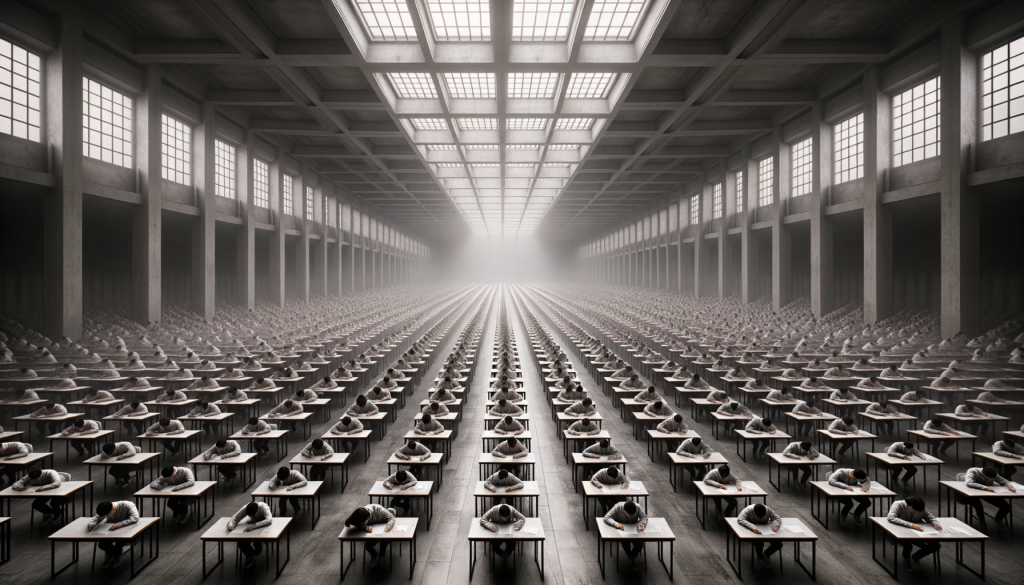
\includegraphics[width=0.45\paperwidth]{07_resources/exam}}
        \put(0.5\paperwidth, 0){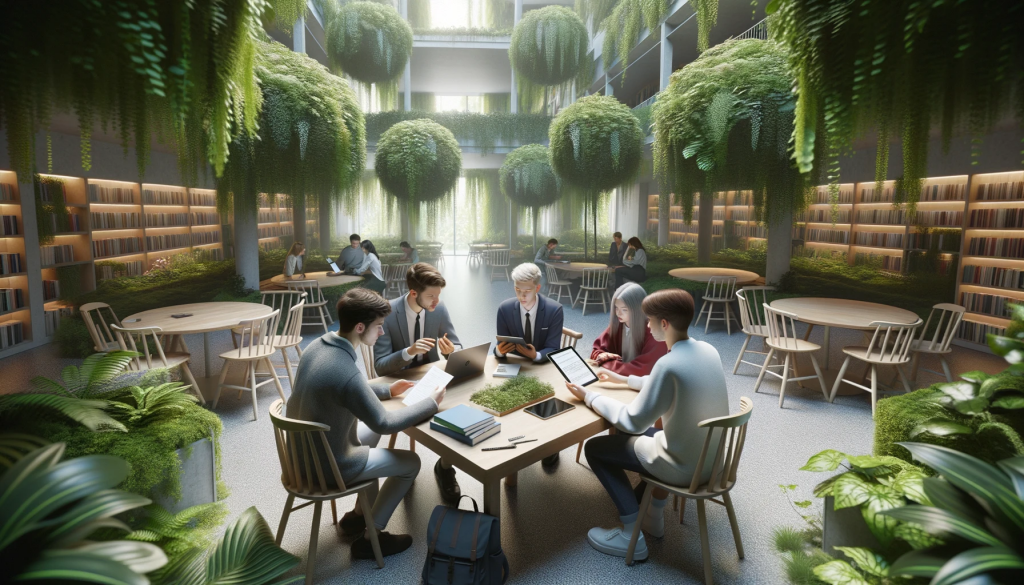
\includegraphics[width=0.45\paperwidth]{07_resources/study_group}}
    \end{picture}
    
    \hspace{17em} To: Tests can be a helpful tool for \positive{improving} learning
\end{frame}


\section{Advantages}
\begin{frame}{Advantages}

    \begin{itemize}
        \item \positive{Strengthens memory}
        \item \positive{Shows gaps in knowledge} ($\rightarrow$ Combats Illusions of Knowing)
        \vspace{1em}
        \item Should be \red{primary study strategy}
        \begin{itemize}
            \item In combination with the other strategies we will cover on the following slides...
        \end{itemize}
    \end{itemize}
\end{frame}


\section{Implementation}
\begin{frame}{Implementation}
    \begin{itemize}
        \item \red{Flashcards}
        \begin{itemize}
            \item Physical
            \item Digital
            \begin{itemize}
                \item Anki (\url{https://apps.ankiweb.net/})
                \item Phase 6 (\url{https://www.phase-6.de/}))
                \item ...
            \end{itemize}
        \end{itemize}
        \item \red{Questions + Answers}
        \begin{itemize}
            \item Physical
            \item Digital 
            \begin{itemize}
                \item Notion (\url{https://www.notion.so/product})
                \item Obsidian (\url{https://obsidian.md/})
                \item RemNote (\url{https://www.remnote.com/computer-science})
            \end{itemize}
        \end{itemize}
    \end{itemize}
\end{frame}


\section{Now You!}
\begin{frame}{Now You!}
    \begin{itemize}
        \item \emph{What would you write on a simple flashcard to test yourself on the topic of retrieval?} \pause
        \begin{itemize}
            \item \emph{Front: What is \red{Retrieval}?}
            \item \emph{Back: A very effective learning strategy where you answer a question instead of simply reading the solution}
        \end{itemize}
        \item \emph{Which of your courses benefit most from implementing Retrieval?}
        \item \emph{How exactly do you want to implement Retrieval into your study routine?}
    \end{itemize}
\end{frame}


\section*{Outlook}
\begin{frame}{Outlook}
    \begin{enumerate}
        \item \positive{Introduction}
        \vspace{.5em}
        \item \positive{Illusions of Knowing}
        \item \positive{Understanding the Brain}
        \item \positive{Learning}
        \item \positive{Desirable Difficulties}
        \item \positive{Effective vs. Ineffective Learning Strategies}
        \vspace{.5em}
        \item \positive{Retrieval}
        \item Next: \red{Spacing}
        \item \grey{Variation and Interleaving}
        \item \grey{Mental Models}
        \item \grey{Memory Cues}
    \end{enumerate}
\end{frame}

\thankyou{Happy Learning!}{sven.ligensa@uni-muenster.de}

\sources

\end{document}
